\documentclass[10pt,a4paper]{article}
\usepackage[utf8]{inputenc}
\usepackage{amsmath}
\usepackage{amsfonts}
\usepackage{amssymb}
\usepackage{graphicx}
\usepackage[swedish]{babel}
\usepackage[utf8]{inputenc}

\graphicspath{}

\author{
  \texttt{Sebastian Bångerius}
}

\begin{document}
\pagenumbering{gobble}

\title{Saker vi ska kunna till tentorna}
\maketitle

\cleardoublepage

\tableofcontents

\clearpage
\section{Disclaimer}
Detta dokument ser snyggt och seriöst ut för att det är skrivet i Latex. Lita inte på att allt står med. Jag är inte så seriös som jag framställer mig.

\section{Flervariabelanalys}
Vi har tagit upp områden såsom \textit{Flervariabelgränsvärden}, \textit{Partialderivator}, \textit{Partiella differetialekvationer}, \textit{Kedjeregeln} , \textit{}, \textit{Gradienter}, \textit{Funktionaldeterminanter} och \textit{Dubbel-/Trippelintegraler} samt \textit{Medelvärdessatsen}

\subsection{Triangelolikheten}
\begin{equation}
\left|x+y\right|\leq\left|x\right|+\left|y\right|
\end{equation}
\begin{flushleft}
Triangelolikheten behandlar vektorer av olika grader. Kan effektivt användas för att stänga in flervarabelfunktioner.
\end{flushleft}
\begin{center}
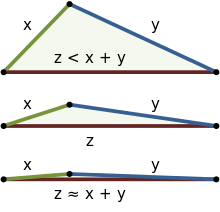
\includegraphics[scale=0.5]{triangelolikhet}
\end{center}

\subsection{Kedjeregeln}
Kedjeregeln används för att kunna bestämma derivator vid variabelbyten. I formuleringen nedan är $f$ en funktion av $x$ och $y$ enligt $f(x(u,v),y(u,v))$. Tänk på att $x=v$ \underline{ej} medför att $\frac{\partial f}{\partial x} = \frac{\partial f}{\partial v}$.
\begin{equation}
\frac{\partial f}{\partial u}=\frac{\partial f}{\partial x}\cdot \frac{\partial x}{\partial u} + \frac{\partial f}{\partial y} \cdot \frac{\partial y}{\partial u}
\end{equation}
\begin{equation}
\frac{\partial f}{\partial v}=\frac{\partial f}{\partial x}\cdot \frac{\partial x}{\partial v} + \frac{\partial f}{\partial y} \cdot \frac{\partial y}{\partial v}
\end{equation}

\end{document}